

\documentclass{article}


% Language setting

% Replace `english' with e.g. `spanish' to change the document language

\usepackage[english]{babel}


% Set page size and margins

% Replace `letterpaper' with`a4paper' for UK/EU standard size

\usepackage[letterpaper,top=2cm,bottom=2cm,left=3cm,right=3cm,marginparwidth=1.75cm]{geometry}


% Useful packages

\usepackage{amsmath}

\usepackage{graphicx}

\usepackage[colorlinks=true, allcolors=blue]{hyperref}


\title{COMP 562 Final Project Report}

\author{Andrew Shooman, Ameer Qaqish, Hugh Williamson, Jack Herbert}


\begin{document}

\maketitle

\section{Introduction}

According to the CDC, stroke is the fifth leading cause of death for Americans. It accounts for 1 in every 6 deaths from cardiovascular disease in the US. Additionally, nearly 795,000 people in the US experience a stroke each year. About 77 percent of these are first time strokes, meaning awareness of risk can help to prevent many of these occurrences. For our project we chose to investigate the characteristics and variables that are associated with susceptibility to stroke. By identifying the characteristics that are associated with higher risk of stroke through different models, we hope to gain insight on how to predict strokes. This data is especially useful for practitioners or even the individuals themselves to assess susceptibility to stroke. Addressing the specific variables that are identified as indicators could prevent a significant number of first time cases we see today. Recommendations based on our results could also save practitioners, patients, and individuals time and money. 


\section{Relevant Work}

Classifying rare events is a difficult problem that is especially prevalent in the medical field. Occurrence of stroke is an example of such a rare event. We examine a dataset to gain insight on what models do well in predicting strokes.

\section{Approach}

\subsection{The Dataset}
The dataset we examined has $5110$ samples and has the following variables:

\begin{figure}[h]
\caption{Summary of variables in the dataset.}
\centering
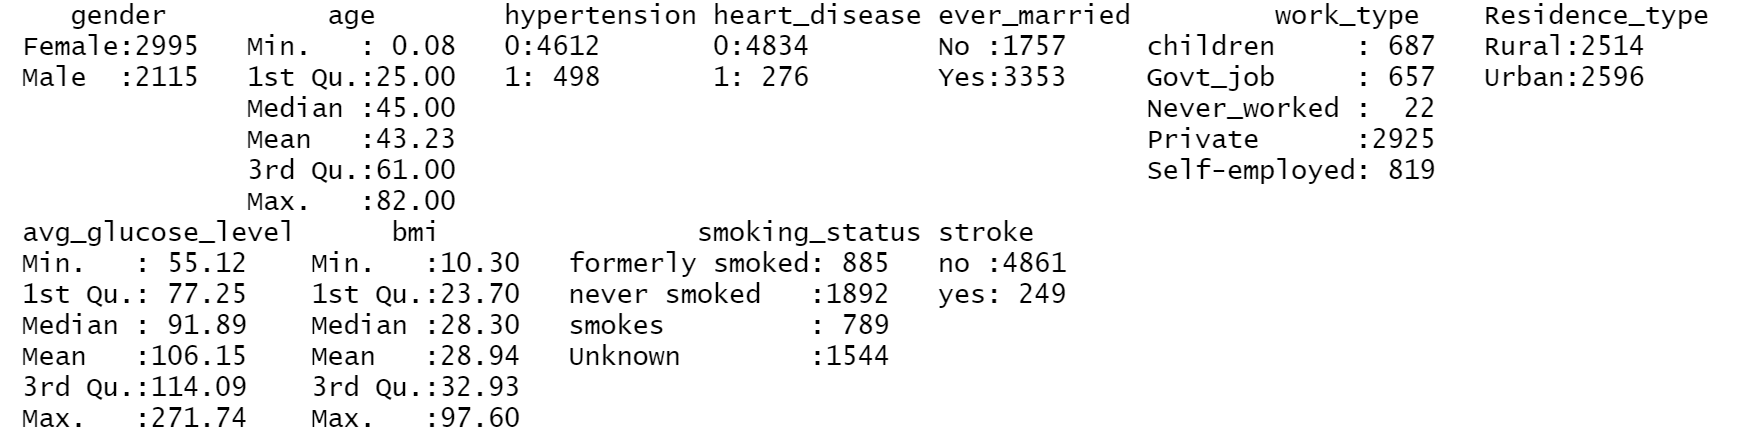
\includegraphics[width = \textwidth]{covariates.png}
\end{figure}

We used the stroke variable as the outcome, and the rest of the variables as covariates in our analysis. In the dataset, $4\%$ of the samples had a missing value for bmi. We imputed these values using a linear regression of bmi on the rest of the variables. Our goal was to find a model that can accurately predict the stroke variable from the other variables. 

\subsection{Model Fitting}
We split the data set into a training set containing $80\%$ of the data, and a test set containing $20\%$ of the data. The split was done randomly. We fit the following models on the training set: logistic regression, support vector machine with linear kernel, $k$-nearest neighbors, random forest, and stochastic gradient boosting. 

Since only $5\%$ of the samples had a stroke, we chose to use Cohen's unweighted Kappa statistic as a metric for choosing the tuning parameters for all the models we fitted. We now explain precisely how we chose the hyperparameters for each model. Logistic regression had no hyper-parameters. For the support vector machine, we chose the cost hyperparameter to be $C = 1$. For the $k$-nearest neighbors, we chose the $k$ hyperparameter from the set $\{5, 7, 9\}$. For each $k \in \{5, 7, 9\}$ we did cross validation with $5$ folds repeated $3$ times and computed the average value of the Kappa statistic when making predictions using the $k$-nearest neighbor algorithm with $k$ neighbors using a threshold of $0.5$ for acceptance (meaning sample $i$ is classified as having a stroke when the probability $p_i$ outputted by the model for this sample is greater than $0.5$). We chose $k$ for which the $k$-nearest neighbor produced algorithm produced the largest average value of the Kappa statistic. This was $k = 5$. For the random forest model, we used $500$ trees. For the number $m$ of variables randomly sampled as candidates at each split, we chose $m$ from the set $\{2, 8, 15\}$ using the same procedure as for choosing $k$ in the $k$-nearest neighbors algorithm. We chose $m = 15$. For the stochastic gradient boosting model hyperparameters, we chose the max tree depth from $\{1, 2, 3\}$, number of trees from $\{50, 100, 150\}$, a shrinkage value of $0.1$, and a minimum terminal node size of $10$. We chose the max tree depth to be $2$ and the number of trees to be $150$ using the same procedure as for choosing $k$ in the $k$-nearest neighbors algorithm.

After each model was trained, the output of each model was a probability $p_i$ for each sample to have a stroke. In order to make predictions, for each model we chose a threshold probability $t$ and considered $p_i > t$ as a prediction that sample $i$ had a stroke, and $p_i \leq t$ as a prediction that sample $i$ did not have a stroke. For each model (so different models had different thresholds), the threshold $t$ was chosen to maximize Cohen's unweighted Kappa statistic when doing prediction on the training set. 

\section{Results}

The logistic regression model coefficients are displayed in figure 2.

\begin{figure}[h]
\caption{Logistic regression model coefficients.}
\centering
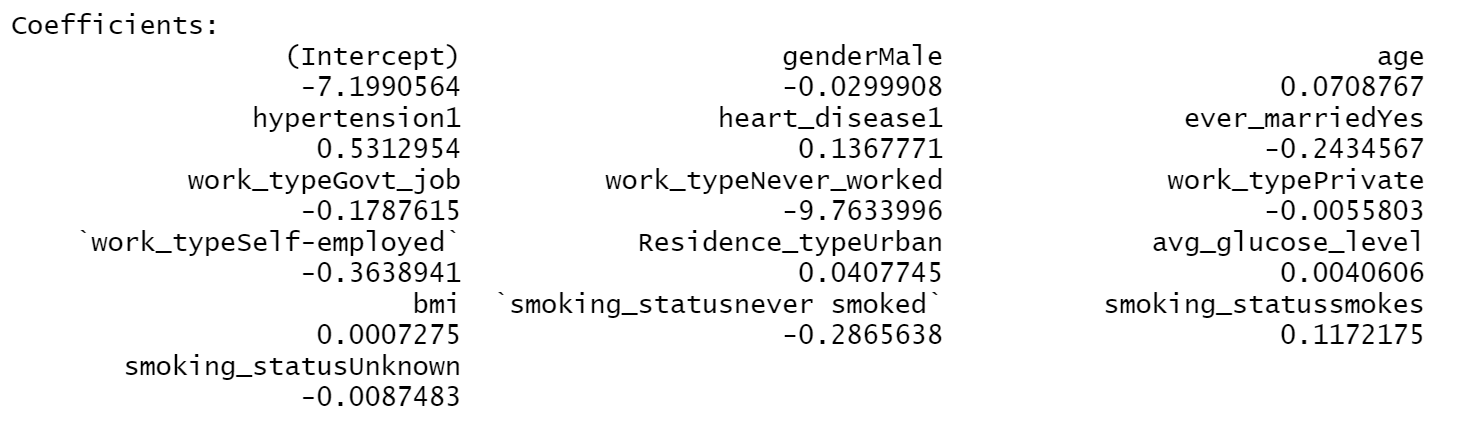
\includegraphics[width = \textwidth]{logRegCoeffs.png}
\end{figure}

From these coefficients, we see that having hypertension, having heart disease, and smoking were the most influential covariates that were positively associated with stroke according to the model. We also see that never working, never smoking, and having ever been married were the most influential covariates that were negatively associated with stroke. We ran each model on the test set. The resulting confusion matrices for each of the models are displayed in figures $3, 4, 5, 6, 7$.

\begin{figure}[h]
\caption{\textbf{Logistic Regression}}
\centering
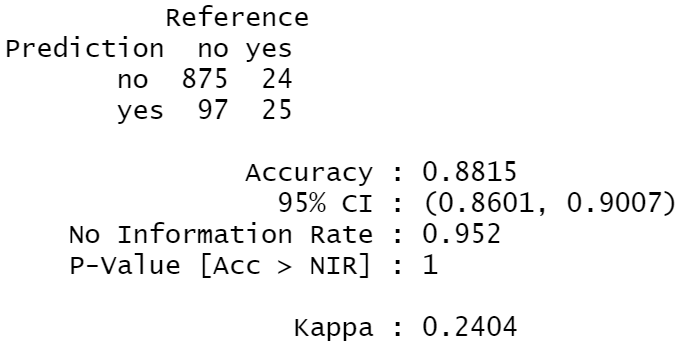
\includegraphics[width = 0.5\textwidth]{logRegCmtx.png}
\end{figure}

\begin{figure}[h]
\caption{\textbf{Support vector machine}}
\centering
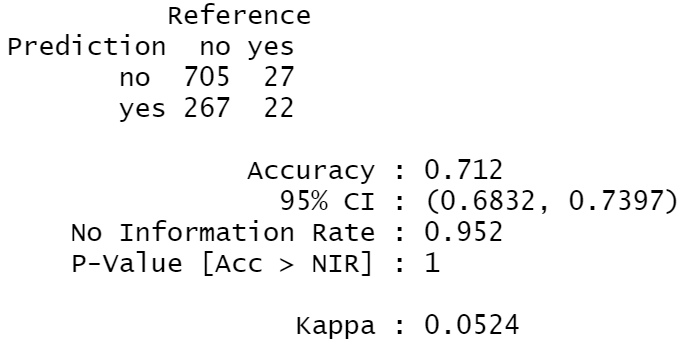
\includegraphics[width = 0.5\textwidth]{svmCmtx.png}
\end{figure}

\begin{figure}[h]
\caption{\textbf{$k$-Nearest Neighbors}}
\centering
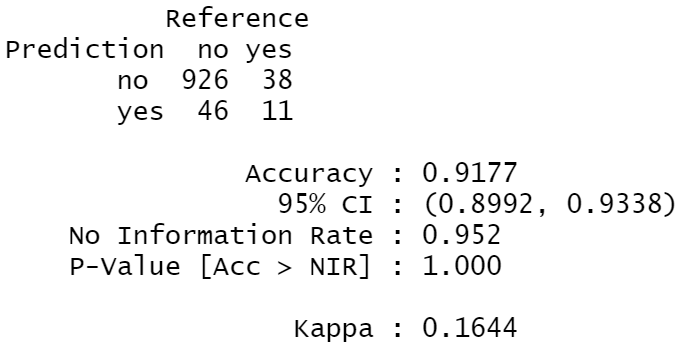
\includegraphics[width = 0.5\textwidth]{knnCmtx.png}
\end{figure}

\begin{figure}[h]
\caption{\textbf{Random forest}}
\centering
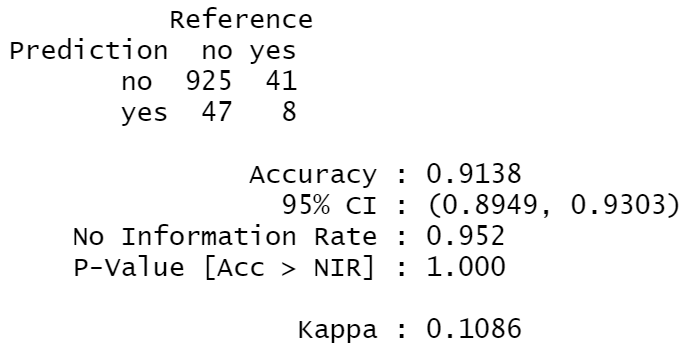
\includegraphics[width = 0.5\textwidth]{rfCmtx.png}
\end{figure}

\begin{figure}[h]
\caption{\textbf{Stochastic Gradient Boosting}}
\centering
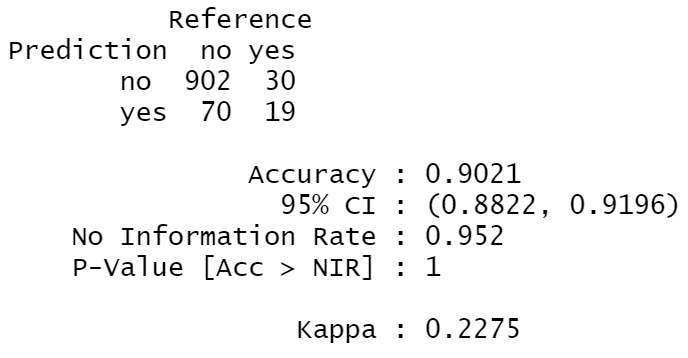
\includegraphics[width = 0.5\textwidth]{gbmCmtx.png}
\end{figure}

\section{Conclusion}

From the confusion matrices, we see that all the models had relatively poor sensitivity compared to specificity, that is, the models struggled to classify those who had a stroke as having a stroke. This is probably due to the low proportion of positive examples in the dataset. Out of all the models, the logistic regression had the highest sensitivity and kappa statistic, although the logistic regression model had the second highest number of false positive predictions after the svm model.  

\section{Further Considerations}
The classification of strokes was difficult mainly due to the low number of positive examples in the dataset. Obtaining more data and using more covariates could help improve the accuracy of the models. Different ways of choosing the hyper-parameters may also give better results.

One thing we observed in the data set is that the $4\%$ of individuals with missing bmi values had strokes at a higher proportion ($20\%$) than those with bmi values. Since the source of the data is confidential, we do not know the reason for this.

\begin{thebibliography}{9}

\bibitem{dataset} 
Stroke Prediction Dataset,
\\\texttt{https://www.kaggle.com/fedesoriano/stroke-prediction-dataset}
\end{thebibliography}

\end{document}
